\section{Persistant Data Management}
Data of most entities in the \texttt{DriveIT System} needs to be stored persistently to avoid data loss if the system crashes and ensure that users can expect to resume work from the point where they last left.
The EntityFramework sub system stores this data using an SQL database hosted online. 
It stores the following entities:
\begin{itemize}
	\item \textbf{Car:} Representing a used car. Cars are read, modified and deleted in every sub system in the \texttt{DriveIT System}.\\
	Cars have many attributes, all describing the properties of the car. Cars are referenced in many other entities in the storage system, but do not reference other entities themselves.\\
	\item \textbf{Customer:} Representing a potential buyer of cars. Customers are read by some parts of the system, but only modified and deleted in certain authorized instances. \\
	Customers have few attributes describing the person acting as the customer. Customers are referenced in some entities in the storage system, but do not reference other entities themselves.
	\item \textbf{Employee:} Representing a salesman of cars. Employees are read by some parts of the system, but only modified and deleted in certain authorized instances. \\
	Employees have few attributes describing the person selling cars. Employees are referenced in some entities in the storage system, but do not reference other entities themselves.
	\item \textbf{Sale:} Representing a sale of a car. Sales are read by some parts of the system, but only modified and deleted in certain authorized instances. \\
	Sales have few attributes describing the specific sale, but mainly reference other entities. A given sale references an \texttt{Employee}, a \texttt{Car} and a \texttt{Customer}.
	\item \textbf{Comment:} Representing a comment on a car. Comments are read by some parts of the system, but only modified and deleted in certain authorized instances. \\
	Comments have few attributes describing the specific comment, but mainly reference other entities. A given comment references a \texttt{Car} and a \texttt{Customer}.
	\item \textbf{ContactRequest:} Representing a request for contact by an \texttt{Employee} about a \texttt{Car}. ContactRequests are read by few parts of the system and only modified and deleted in certain authorized instances. \\
	ContactRequests have one attribute describing the specific request, but mainly reference other entities. A given ContactRequest references a \texttt{Car} , an \texttt{Employee} and a \texttt{Customer}.
\begin{figure}[h!]
	\centering
		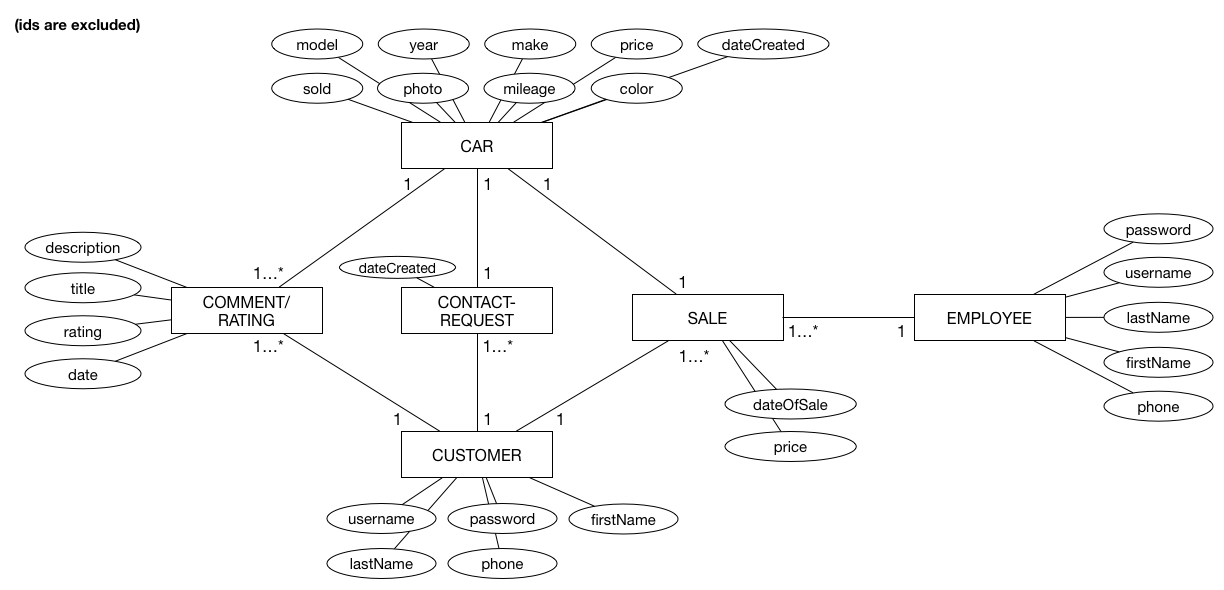
\includegraphics[scale=0.30]{Figures/PersistentDataModel}\\
		% place the figure in the Figures folder (located with the main file)
		% you need to fix the scale a few times to get it right, but latex does not compress so one can always zoom in to see details.
	\caption{The Persistent Data Model.}
\end{figure}